\documentclass{article}
\usepackage[utf8]{inputenc}
\usepackage{graphicx}
\usepackage{amsmath}
\usepackage{hyperref}
\usepackage{float}
\usepackage{geometry}
\usepackage{titling}
\usepackage{amssymb}
\usepackage{abstract}
\usepackage{multicol}
\usepackage{biblatex}
\usepackage{listings} % Add the missing LaTeX package
\usepackage{subcaption}



% \usepackage{quantikz}


\addbibresource{bibliography.bib}
\geometry{a4paper, left=2cm, right=2cm, top=2cm, bottom=2cm}


\usepackage{fancyhdr}

\pagestyle{fancy}
\fancyhf{}
\lhead{M1 PAD \\ \rule{\textwidth}{0.4pt} \\ Projet de M1}
\rhead{MU4PYD? \\ \rule{\textwidth}{0.4pt} \\ 2023-2024}
\renewcommand{\headrulewidth}{0pt}

\begin{document}

\title{Projet de M1 - Optimisation quantique}
\author{Martin PUJOL \\ martin.pujol@etu.sorbonne-universite.fr}
\date{}

\maketitle
\thispagestyle{fancy}

\begin{abstract}

Ce projet bibliographique souhaite succintement présenter les principes fondateurs derrières l'ordinateur quantique, aborder la notion de qubit, les façons d'en produire et les problèmes liés à leurs utilisations.
Par la suite, le projet se veut plus ludique en formalisant un probleme d'optimisation (simpiste) et en le résolvant à l'aide d'un ordinateur quantique.

\textbf{Mots clés : Informatique Quantique, Qubit, Optimisation } 

\end{abstract}

\begin{multicols}{2}

\section{Qu'es ce qu'un qubit ?} 
\subsection{Definition}

Un qubit est la contraction de "quantum bit", c'est l'unité de base de l'informatique quantique.
Notre approche de physicien pourrait simplement appeler cette unité un système quantique à deux niveaux.
En effet, un qubit est un système quantique qui peut être dans deux états de base, noté $\left|0\right>$ et $\left|1\right>$.
Pour définir l'état de ce qubit on a alors besoin de deux nombres complexes $a$ et $b$ tel que $a^2 + b^2 = 1$.
On peut écrire l'état du qubit comme suit :
\begin{equation}
\left|\psi\right> = a\left|0\right> + b\left|1\right>
\end{equation}

Que l'on représente communément sous la forme d'un vecteur colonne :

\begin{equation}
\left|\psi\right> = \begin{pmatrix} a \\ b \end{pmatrix}
\end{equation}

Et qui s'illustre sur la sphère de Bloch :

\begin{figure}[H]
    \centering
    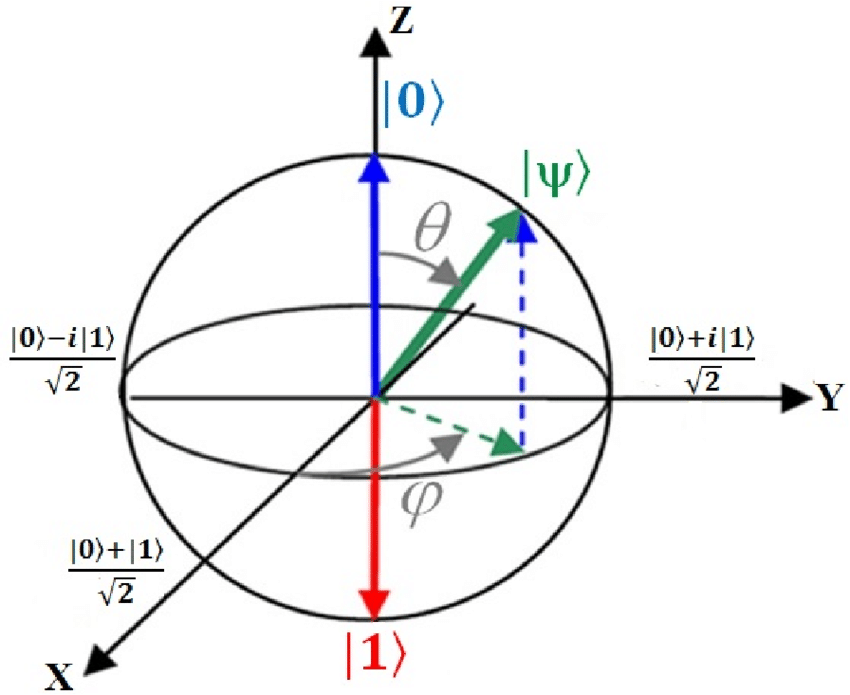
\includegraphics[width = \columnwidth]{fig/bloch_sphere.png}
    \caption{Sphère de Bloch}
    \label{fig:sphere_de_bloch}
\end{figure}

En sachant qu'un état quantique est défini à un facteur près, nous pouvons ainsi veiller à ce que "a" soit réel. Cette caractéristique nous permet alors de représenter l'état d'un qubit en trois dimensions. En ajoutant la contrainte sur sa norme, nous pouvons visualiser cet état sur la sphère de Bloch  (voir la figure \autoref{fig:sphere_de_bloch}).

\subsection{Mesure d'un qubit}

La mesure d'un qubit est un peu particulière, en effet, on ne peut pas mesurer un qubit sans détruire la superposition.
La mesure d'un qubit est un processus irréversible qui consiste à projeter l'état du qubit sur l'un des deux états de base.
On peut alors définir deux opérateurs de projection $\left|0\right>\left<0\right|$ et $\left|1\right>\left<1\right|$.
Ainsi on définit la probabilité de mesurer l'état $\left|0\right>$ comme suit :

\begin{equation}
    P(\left|0\right>) = \left<\psi\right|\left|0\right>\left<0\right|\left|\psi\right> = a^2
\end{equation}

Et la probabilité de mesurer l'état $\left|1\right>$ comme suit :

\begin{equation}
    P(\left|1\right>) = \left<\psi\right|\left|1\right>\left<1\right|\left|\psi\right> = b^2
\end{equation}

On voit déjà que l'on ne pourra pas mesurer l'état de notre qubit pendant notre calcul, tout le challenge résidera alors dans le fait de pouvoir exploiter les propriétés quantiques de notre qubit afin de le manipuler sans le mesurer. Et c'est seulement à la fin de ces manipulations que l'on pourra mesurer notre qubit pour obtenir le résultat de notre calcul en utilisant entre autre les opérateurs de projections précédemment définis.

\subsection{Superposition et intrication de qubits}

Après avoir introduit la notion de qubit, on a du mal a voir comment on pourrait extraire une quelconque puissance de calcul de ce système. 
On peut d'abord par analogie avec le bit classique se demander que se passerait-il en utilisant N qubits. 
On aurait alors un systeme quantique à $2^N$ états de base, et donc un système quantique qui pourrait être dans une superposition de $2^N$ états différents.
Voici par exemple l'etat d'un système à 3 qubits :

\begin{align}
    \left|\psi\right> = & a\left|000\right> + b\left|001\right> + c\left|010\right> \nonumber \\
    & + d\left|011\right> + e\left|100\right> + f\left|101\right> \nonumber \\
    & + g\left|110\right> + h\left|111\right>
\end{align}

Que l'on peut représenter sous la forme d'un vecteur colonne :

\begin{equation}
    \left|\psi\right> = \begin{pmatrix} a \\ b \\ c \\ d \\ e \\ f \\ g \\ h \end{pmatrix}
\end{equation}


Ainsi, on remarque que 3 qubits portent une information qui est de taille $2^3 = 8$ variables continues.

C'est bien cette superposition qui nous intéresse, en effet, on peut alors exploiter cette superposition pour effectuer des calculs. Par exemple, "explorer" les différents états superposés pour trouver la solution d'un problème d'optimisation.
Cet espace très large de superposition va nous permettre d'encoder des informations de façon très compacte et ainsi effectuer des calculs seulement par la mesure d'états minutieusement préparés.
Une seconde notion très utile va nous permettre de reduire l'espace des états de notre système, il s'agit de l'entrelacement ou intrication de qubits.
En effet, on peut préparer des états quantiques qui ne peuvent pas être décrits comme la superposition de deux états quantiques indépendants. 
Par exemple les états de Bell :

\begin{equation}
    \left|\psi\right> = \frac{1}{\sqrt{2}}\left(\left|00\right> + \left|11\right>\right)
\end{equation}

\begin{equation}
    \left|\psi\right> = \frac{1}{\sqrt{2}}\left(\left|00\right> - \left|11\right>\right)
\end{equation}

\begin{equation}
    \left|\psi\right> = \frac{1}{\sqrt{2}}\left(\left|01\right> + \left|10\right>\right)
\end{equation}

\begin{equation}
    \left|\psi\right> = \frac{1}{\sqrt{2}}\left(\left|01\right> - \left|10\right>\right)
\end{equation}

En effet, si on mesure l'un des qubits de ces états, on connait alors l'état de l'autre qubit.

A ce niveau, l'idée du calculs parrait encore très abstraite, surtout pour l'auteur !
Heuresement, après avoir aborder les facons de produire un qubit nous allons ensemble encoder un problème d'optimisation et le résoudre à l'aide d'un ordinateur quantique.



\section{Comment produire un qubit et agir sur son états ?}

Un qubit étant un système quantique à deux niveaux, il existe une multitude de moyens de produire un qubit pouvant reposer sur des propriétés physiques très différentes.
Ainsi on peut utiliser des atomes, des ions, des photons, des défauts de spin, des boites quantiques, des molécules, des supraconducteurs et bien d'autres.
Il est donc très difficile d'être exhausif mais l'industrie et le monde de la recherche se concentre sur quelques technologies qui semblent être les plus prometteuses.
Ces technologies sur lesquelles nous nous concenterons qui sont les qubits supraconducteurs, les qubits à ions piégés et les qubits à photons. 
Elles ne sont pas par hasard les plus prometteuses, un qubit n'est pas parfait et on veut d'abord que ce qubit soit très stable, c'est à dire que l'on puisse conserver son état le plus lontemps possible. On parle alors de cohérence du qubit.
On veut aussi que ce qubit soit très facile à produire et à manipuler. On parle alors de scalabilité du qubit.
Enfin certaine technologies facilitent l'utilisation de certaine propriétés quantiques comme l'entrelacement de qubits.


\subsection{Les qubits à ions piégés}

Les qubits à ions piégés sont constitutés d'ions hydrogénoides qui sont piégés dans un champ électromagnétique.
Pour ces qubits, le systeme physique a considerer est le niveau d'énergie de l'electron. 
On va donc d'abord refroidir ces ions pour les rendre très proche du zéro absolu, puis on va les piéger dans un champ électromagnétique en utilisant un quadrupole comme suit :


\begin{figure}[H]
    \centering
    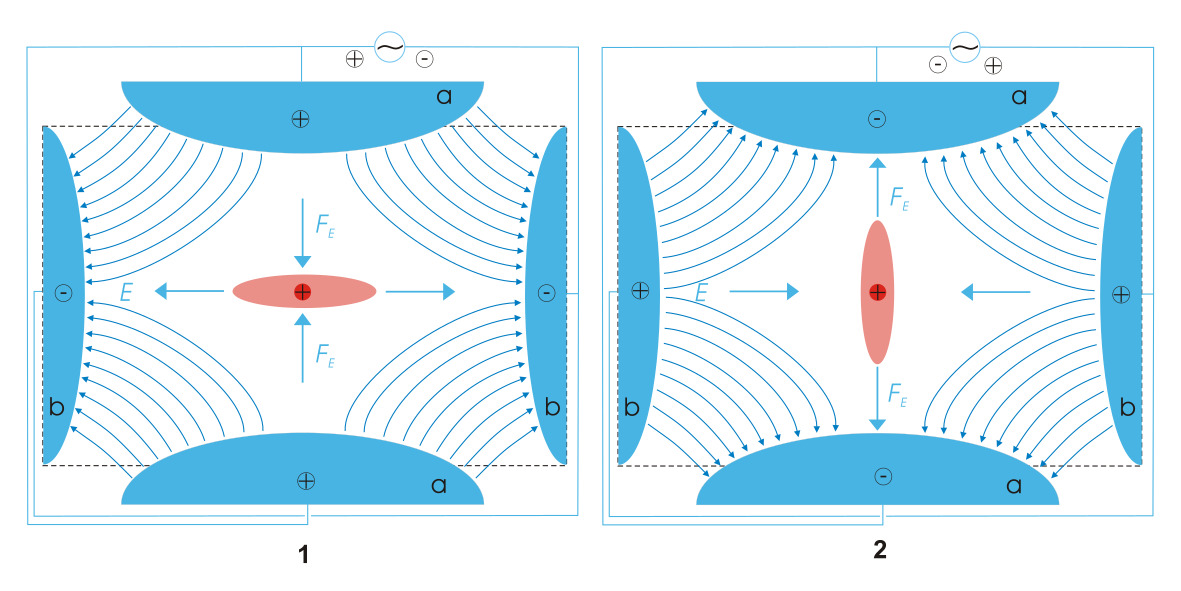
\includegraphics[width = \columnwidth]{fig/Paul-Trap.png}
    \caption{Piège de Paul}
    \label{fig:Paul_Trap}
\end{figure}


On peut alors utiliser des lasers pour agir sur l'état d'énergie de l'electron.
% Ces qubits sont très prometteurs car ils sont très stables et sont donc très faciles à manipuler.
% Cependant, ils sont très difficiles à produire et à manipuler.
% C'est pour cela que les qubits à ions piégés sont très utilisés pour les applications industrielles mais ne sont pas encore utilisés pour les expériences de preuve de concept.

Les entreprises telles que Pasqal et QuEra (\cite{wintersperger_neutral_2023}, \cite{noauthor_building_nodate}) ont décider de développer des ordinateurs quantiques basés sur cette technologie.
Ils utilisent en particulier les atomes de Rydberg, l'electron de ces atomes hydrogénoides ont la spécificité d'occuper la couche de valence à une distance moyenne très éloigné du noyeau, ce qui les rends très sensible aux champs électromagnétiques et qui facilite aussi l'intrication de ces qubits.


L'Hamiltonien d'un atome de Rydberg peut être représenté comme suit:

$$
\hat{H}_0 = -\frac{\hbar^2}{2m}\nabla^2 - \frac{e^2}{4\pi\epsilon_0 r}
$$

où $m$ est la masse de l'électron, $\hbar$ est la constante de Planck réduite, $e$ est la charge de l'électron, $\epsilon_0$ est la permittivité du vide, et $r$ est la distance de l'électron au noyau.

Si l'on ne considère que deux niveaux d'énergie, le niveau fondamental et un niveau excité. Si on note ces deux niveaux par $|g\rangle$ et $|e\rangle$, la matrice de l'Hamiltonien réduite à ces deux niveaux est :

$$
\hat{H} = \begin{pmatrix}
E_g & \Omega/2 \\
\Omega/2 & E_e
\end{pmatrix}
$$

où $E_g$ et $E_e$ sont les énergies des niveaux $|g\rangle$ et $|e\rangle$, et $\Omega$ est la fréquence de Rabi, qui est proportionnelle à l'amplitude du champ électromagnétique appliqué.

Ces formules sont une simplification et l'Hamiltonien réel d'un atome de Rydberg peut être beaucoup plus complexe, en raison des interactions entre les différents électrons et du couplage avec le champ électromagnétique. De plus, la matrice de l'Hamiltonien dépend du choix des niveaux d'énergie utilisés pour former le qubit.


\subsection{Les qubits supraconducteurs}
Les qubits supraconducteurs sont des circuits électriques refroidis à des températures extrêmement basses afin de les rendre supraconducteurs. 
À de telles températures, ces circuits perdent leurs résistances électriques, ce qui est rendu possible par la formation de paires de Cooper, constituées de deux électrons agissant comme des bosons. 
Dans ces matériaux, tous les électrons peuvent potentiellement former ces paires de Cooper et partager le même état quantique, permettant ainsi la création de qubits sans nécessairement recourir à un seul atome.


On considère donc un circuit linaire LC, où L est l'inductance et C la capacité. 

\begin{figure}[H]
    \centering
    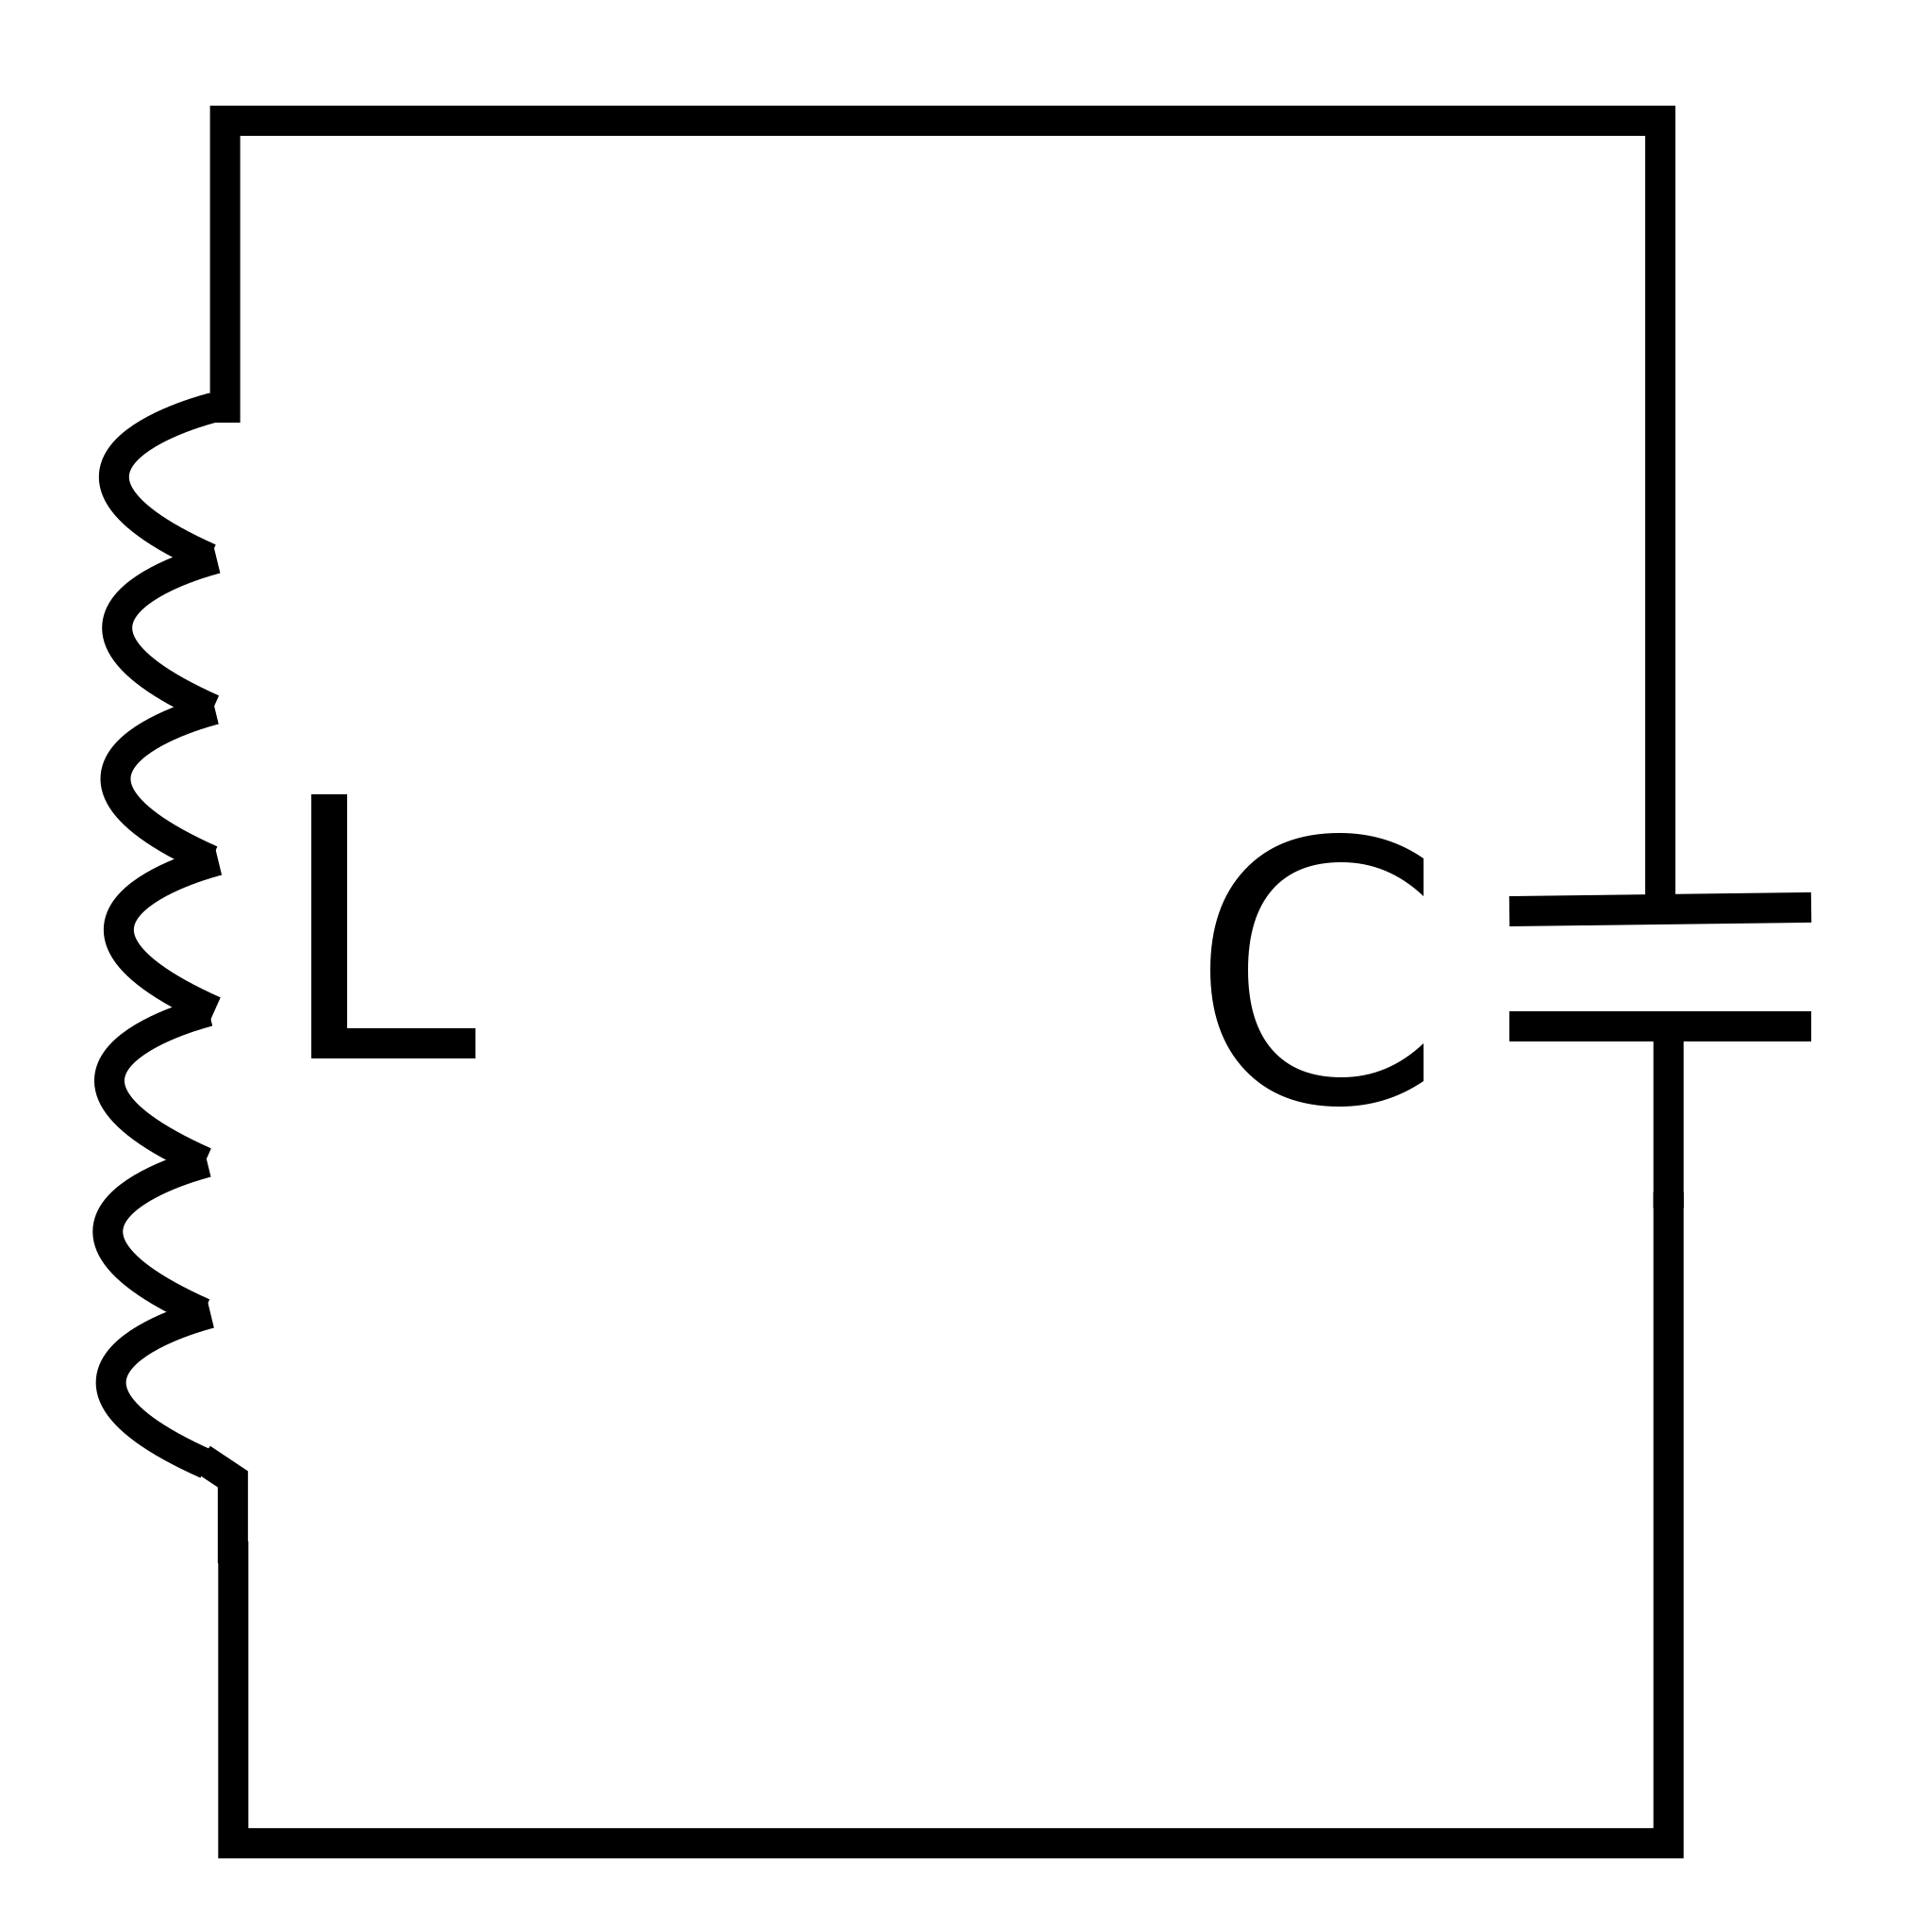
\includegraphics[width = 0.7\columnwidth]{fig/circuit_LC.png}
    \caption{Circuit LC}
    \label{fig:Circuit_LC}
\end{figure}



On peut alors donner l'Hamiltonien de ce circuit comme suit :

$$
H = \frac{{\hat{Q}^2}}{{2C}} + \frac{{\hat{\Phi}^2}}{{2L}}
$$

L'hamiltonien quantifié ci-dessus est généralement écrit sous une forme plus conviviale en utilisant la charge réduite $\hat{n}=\hat{Q}/2e$ et la phase $\hat{\phi}=2\pi\hat{\Phi}/\Phi_0$, où $\Phi_0=h/2e$ est le quantum de flux, correspondant aux opérateurs pour le nombre de paires de Cooper et la phase à travers la jonction Josephson, respectivement. Ensuite, l'hamiltonien quantifié devient

$$
H = 4E_c\hat{n}^2 - E_L\frac{d^2}{d\hat{\Phi}^2}
$$


Un qubit représente alors une portion de matériau où tous les électrons partagent le même état quantique.
Du fait que les électrons se comportent comme des oscillateurs harmoniques (approximativement) dans le matériau, il est possible de s'intéresser à deux niveaux d'énergie de ces oscillateurs pour la manipulation quantique.

Un aspect intéressant est l'effet Josephson, qui résulte de la nature macroscopique et continue de la fonction d'onde des paires de Cooper. Cela signifie qu'approcher deux boîtes supraconductrices l'une de l'autre peut créer un couplage entre leurs fonctions d'onde, facilitant notamment l'intrication quantique.



Ces circuits sont alors des oscillateurs quantiques qui peuvent être dans deux états de base.
On peut alors utiliser des transistors pour agir sur l'état de ces oscillateurs et ainsi produire des qubits.
% Ces qubits sont très prometteurs car ils sont très faciles à produire et à manipuler.
% Cependant, ils sont très sensibles aux bruits environnementaux et sont donc très difficiles à manipuler sans les détruire.
% C'est pour cela que les qubits supraconducteurs sont très utilisés pour les expériences de preuve de concept mais ne sont pas encore utilisés pour les applications industrielles.

En réalité, les ordinateurs quantiques supraconducteurs tels que ceux produit par IBM et google utilise un circuit particulier nommé Transmon.
\begin{figure}[H]
    \centering
    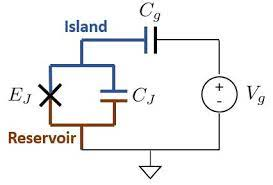
\includegraphics[width = \columnwidth]{fig/transmon_circuit.jpg}
    \caption{Circuit d'un transmon}
    \label{fig:transmon}
\end{figure}

Sans entrer dans les details, ce circuit est analogue à un circuit LC (comme on peut le voir sur la figure \autoref{fig:transmon}) où l'Hamiltonien est donné par :

$$
H = 4E_c\hat{n}^2 - E_J\cos(\hat{\phi})
$$

avec $E_c$ l'énergie de charge, $E_J$ l'énergie de Josephson et $\hat{n}$ et $\hat{\phi}$ les opérateurs pour le nombre de paires de Cooper et la phase à travers la jonction Josephson, respectivement.

Les transmon ont aussi une forme proche d'un oscillateurs quantique, ici on peut voir une figure représentant leurs niveaux d'energie (issus de la documentation IBM \cite{noauthor_introduction_nodate}):

\begin{figure}[H]
    \centering
    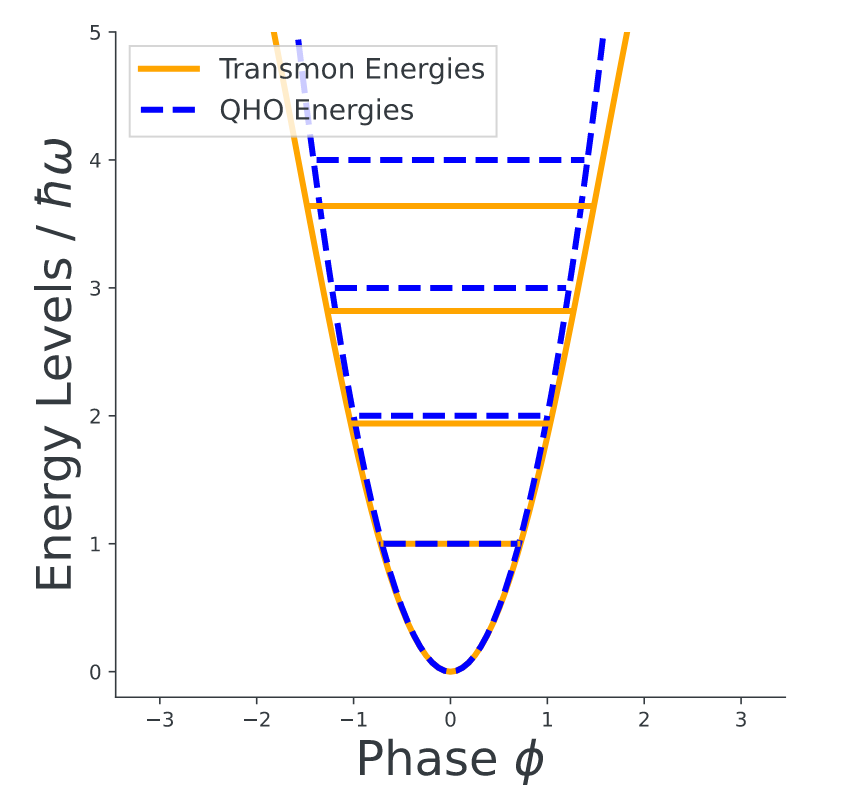
\includegraphics[width = \columnwidth]{fig/transfon.png}
    \caption{Niveaux d'énergie d'un Transmon (IBM)}
    \label{fig:Transmon}
\end{figure}



\subsection{Les qubits à photons}

Finalement, un moyen assez instinctif mais aussi ludique de créer un qubit est d'utiliser des photons.
En effet, on peut décomposer la polarisation d'un photon en deux états de base, noté $\left|0\right>$ et $\left|1\right>$.
On peut alors utiliser des fibres optiques pour agir sur l'état de ces photons et ainsi produire des qubits.

\begin{figure}[H]
    \centering
    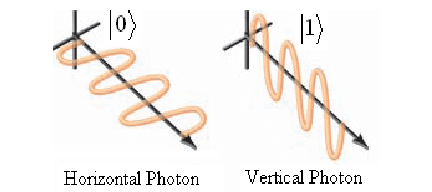
\includegraphics[width = \columnwidth]{fig/Single-photon-qubit.png}
    \caption{Qubit à photons}
    \label{fig:Qubit_a_photons}
\end{figure}

Ici, l'Hamiltonien de notre systeme ne nous interesse pas vraiment car on ne souhaite plus mesurer l'énergie de notre système.

On peut par exemple introduire l'observable $\hat{\sigma}_z = \left|0\right>\left<0\right| - \left|1\right>\left<1\right|$ qui va nous permettre de mesurer l'état de polarisation de notre qubit.

Cette observable traduira alors l'action d'un filtre polarisant sur notre qubit.

\subsection{Quelle technologie choisir ?}

Il est assez difficile de dire quelle technologie est la plus prometteuse. Chaque technologie a ses avantages et ses inconvénients. IBM avec leurs qubits supraconducteurs et Pasqal avec leurs qubits à ions piégés semblent très prometteurs en termes de scalabilité, car ces technologies permettent d'atteindre un grand nombre de qubits. Cependant, il faut prendre en compte le fait qu'appliquer une opération logique sur ces qubits peut modifier l'information et transformer un qubit de l'état $\left|0\right>$ à l'état $\left|1\right>$. La notion de fidélité des portes est donc une question majeure, mais les entreprises ne communiquent pas toujours à ce sujet. En attendant, on peut utiliser plusieurs qubits pour corriger les erreurs de mesure et de manipulation, ce que l'on appelle les codes correcteurs d'erreurs. Par ailleurs, Pasqal ne permet toujours pas d'appliquer des portes logiques sur ses qubits, et il y a d'autres problématiques, par exemple les qubits supraconducteurs à ions piégés permettent l'intrication de proche en proche (spatialement) et donc ne permettent pas d'intriquer des qubits éloignés. D'autres entreprises font des paris différents, notamment Alice et Bob avec leurs qubits de chat, qui se montrent hermétiques à un type d'erreur en particulier. Finalement, pour les ordinateurs à porte quantique, on peut se baser sur deux informations : la fidélité des portes à 2 qubits et le nombre de qubits physiques. De plus, un objectif souhaitable pour la technologie actuelle est d'atteindre le stade de NISQ (Noisy Intermediate-Scale Quantum), où les ordinateurs quantiques pourraient être utilisés pour des applications pratiques malgré les erreurs de mesure et de manipulation. Pour atteindre ce stade, il faudrait avoir plus de 40 qubits physiques avec des portes à 2 qubits de fidélité supérieure à 99,9\%. La figure ci-dessous (\autoref{fig:nisq}) issus de \cite{ezratty_where_2023} permet de visualiser les performances des différentes technologies en fonction du nombre de qubits et de la fidélité des portes à 2 qubits.

\begin{figure}[H]
    \centering
    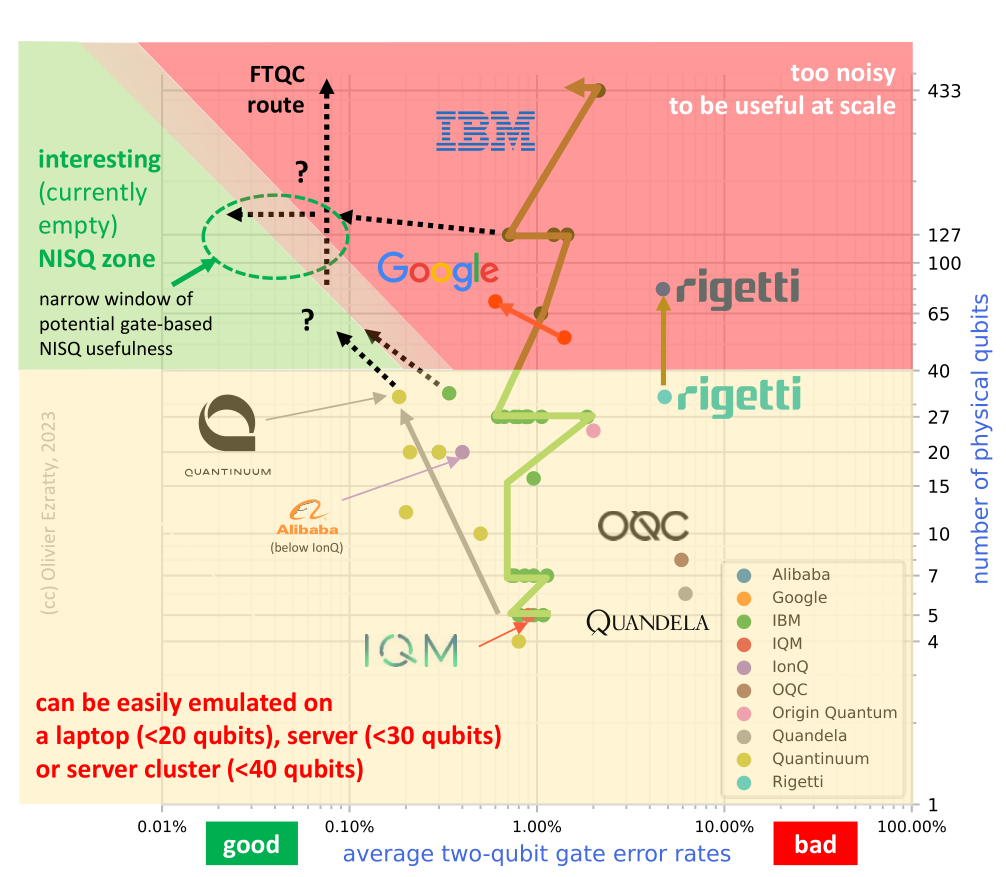
\includegraphics[width = \columnwidth]{fig/NISQ.png}
    \caption{Performance des différentes technologies en fonction du nombre de qubits et de la fidélité des portes à 2 qubits}
    \label{fig:nisq}
\end{figure}



A ce jour, la technologie la plus avancée est celle des qubits supraconducteurs, car IBM et Google ont déjà produit des ordinateurs quantiques avec plus de 50 qubits. Bien que la fidélité de ces portes ne soient pas très élevées, IBM met à disposition différents types de portes ainsi que des codes correcteurs d'erreurs très performants (\cite{bravyi_high-threshold_2024}).

D'un autre côté, les qubits à ions piégés se présentent comme la technologie la plus prometteuse, notamment en raison de leur scalabilité. Des expériences ont montré qu'il est possible de maintenir des lignes de milliers de ces ions, et les efforts de Quantinuum pour proposer des qubits extrêmement stables sont très encourageants.

Avec le dernier article de Quantinuum et Microsoft annonçant un nouveau code d'erreur réduisant les erreurs de 800 fois (\cite{zander_advancing_2024}), il semble que Quantumium pourrait s'imposer comme le leader de l'informatique quantique.

Finalement, il est important de savoir qu'aucun ordinateur quantique n'est identique. Les qubits de chat sont hermétiques à un type d'erreur, les qubits à ions piégés ont des propriétés physiques étonnantes comme le blocage de Rydberg qui introduit des possibilités différentes, et les ordinateurs à photons ont un fonctionnement très différent des autres technologies et pourraient être très utiles pour certaines applications.

\section{Algorithme et Optimisation quantique}

Pour agir sur l'état d'un qubit, on peut utiliser des opérateurs.
Ces opérateur vont traduire l'action d'e mesure physique sur l'état d'un qubit.
Cependant, si on ne s'interesse qu'aux variables qui définissent l'état d'un qubit (les coefficients $a$ et $b$), le systeme physique que l'on utilise n'a plus vraiment d'importance.
En effet, si on utilise un atome de Rydberg, un circuit supraconducteur ou un photon, on peut toujours définir des opérateurs qui vont agir sur l'état de notre qubit de la même manière par exemple un opérateur qui transforme l'état $\left|0\right>$ en $\left|1\right>$ et vice versa.


\subsection{Les portes quantiques}

On va donc pouvoir introduire des portes quantiques qui sont les représentations algébriques des opérateurs qui agissent sur l'état d'un qubit.

\subsubsection{Porte de Pauli}

La porte de Pauli est une porte quantique qui agit sur l'état d'un qubit en le faisant tourner autour de l'axe $x$, $y$ ou $z$.
On peut alors définir les portes de Pauli comme suit :

\begin{equation}
    X = \begin{pmatrix} 0 & 1 \\ 1 & 0 \end{pmatrix}
\end{equation}

\begin{equation}
    Y = \begin{pmatrix} 0 & -i \\ i & 0 \end{pmatrix}
\end{equation}


\begin{equation}
    Z = \begin{pmatrix} 1 & 0 \\ 0 & -1 \end{pmatrix}
\end{equation}

\subsubsection{Porte de Hadamard}

La porte de Hadamard est une porte quantique qui agit sur l'état d'un qubit en le faisant tourner autour de l'axe $x$ et $z$.

\begin{equation}
    H = \frac{1}{\sqrt{2}}\begin{pmatrix} 1 & 1 \\ 1 & -1 \end{pmatrix}
\end{equation}

\subsubsection{Porte de phase}

La porte de phase est une porte quantique qui agit sur l'état d'un qubit en le faisant tourner autour de l'axe $z$.

\begin{equation}
    S = \begin{pmatrix} 1 & 0 \\ 0 & i \end{pmatrix}
\end{equation}


\subsubsection{Porte de CNOT}

La porte de CNOT est une porte quantique qui agit sur l'état de deux qubits en "inversant" l'état du second qubit.

\begin{equation}
    CNOT = \begin{pmatrix} 1 & 0 & 0 & 0 \\ 0 & 1 & 0 & 0 \\ 0 & 0 & 0 & 1 \\ 0 & 0 & 1 & 0 \end{pmatrix}
\end{equation}

Les portes que nous venons de citer sont fondamentales dans le sens que combinés elles permettent de réaliser n'importe quelle opération logique sur l'état de nos qubits.



On va maintenant se demander comment on peut utiliser ces qubits pour effectuer des calculs.
D'abord, il est important de noter qu'il n'existe pas de problème qu'un ordinateur quantique peut résoudre et pas un ordinateur classique.
Cependant, certain problème sont solvable en un nombre d'opérations beaucoup plus faible avec un ordinateur quantique qu'avec un ordinateur classique.
Par exemple, on peut citer l'algorithme de Shor qui permet la factorisation en nombres premier avec un nombre de pas exponentiellement plus faible qu'avec un ordinateur classique.



\subsection{Optimisation quantique}

Une autre facon de mettre à profit les propriétés quantiques de nos qubits est de les utiliser pour résoudre un problème d'optimisation.
En effet, si l'on parvient à faire en sorte que le cout de notre problème d'optimisation correspondent à l'hamiltonien de notre système quantique, alors trouver l'état fondemental de notre système quantique reviendra à résoudre notre problème d'optimisation.

\subsubsection{Theoreme adiabatique}

Une question qui se pose d'abord est comment trouver l'état fondamental associé à notre système quantique. 
C'est ici qu'intervient le théorème adiabatique. Selon ce théorème, si notre système quantique est préparé dans l'état fondamental de son hamiltonien, alors si l'hamiltonien du système change lentement, l'état change afin de rester dans l'état fondamental de l'hamiltonien.

Formellement, si on note $\hat{H}(t)$ l'hamiltonien de notre système quantique à l'instant t, alors si on fait varier $\hat{H}(t)$ de telle sorte que :

\begin{equation}
    \hat{H}(t) = (1-t/T)\hat{H}_0 + (t/T)\hat{H}_f
\end{equation}

Avec $\hat{H}_0$ l'hamiltonien de notre système quantique à l'instant t=0 et $\hat{H}_f$ l'hamiltonien de notre système quantique à l'instant t=T, si T est suffisament grand, alors l'état fondamental de $\hat{H}_0$ évoluera vers l'état fondamental de $\hat{H}_f$.

Cette variation doit respecter :

\begin{equation}
    \tau \gg \frac{\max_{ 0 \leq s \leq 1}  \left| \left\langle \psi_1(s) \left| \frac{\partial \hat{H}(s)}{\partial s} \right| \psi_0(s) \right\rangle \right| }{\min_{0 \leq s \leq 1} \Delta^2(s)} ; s \equiv t 
\end{equation}

\subsubsection{Hamiltonien d'Ising}

Maintenant, nous devons faire en sorte que le coût de notre problème d'optimisation corresponde à l'hamiltonien de notre système.
Nous allons donc encoder notre problème d'optimisation en un hamiltonien d'Ising.

L'hamiltonien d'Ising est donné par :

\begin{equation}
    \hat{H} = -\sum_{i,j} J_{ij}\hat{\sigma}_i^z\hat{\sigma}_j^z - \sum_i h_i\hat{\sigma}_i^z
\end{equation}

Avec $\hat{\sigma}_i^z$ l'observable de Pauli, $J_{ij}$ les poids de couplage entre les spins et $h_i$ les champs magnétiques locaux.


On remarque là qu'il est important que notre Hamiltonien initial ne commute pas avec l'Hamiltonien d'Ising sinon l'état initial serait un etat stationnaire des deux Hamiltonien et donc n'évoluerait pas.




\subsection{Probleme d'optimisation : Le max cut edge}

Le max cut edge est un problème d'optimisation qui consiste à trouver la coupe d'un graphe qui maximise le nombre d'arêtes coupées.
Les information du problèmes sont donc les noeuds et les arêtes entre ses noeuds. 
Il est catégorisé comme NP-Hard ce qui signifie qu'il solvable en un temps exponentiel avec un ordinateur classique. 
Cependant, on peut utiliser un ordinateur quantique pour résoudre ce problème en un temps polynomial.

\begin{figure}[H]
    \centering
    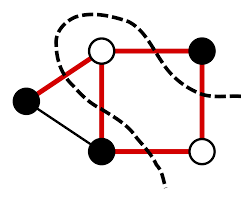
\includegraphics[width = \columnwidth]{fig/Max_Cut.png}
    \caption{Max cut edge}
    \label{fig:Max_cut_edge}
\end{figure}

Voici un exemple pour deux noeuds : 


\begin{figure}[H]
    \centering
    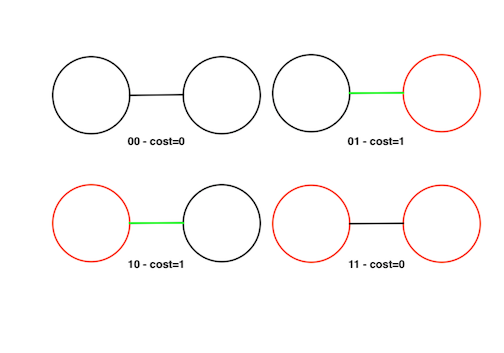
\includegraphics[width = \columnwidth]{fig/02_2_nodes_cuts.png}
    \caption{Max cut edge avec 2 noeuds}
    \label{fig:Max_cut_edge_2}
\end{figure}

Et ici, un exemple avec 3 noeuds :
\begin{figure}[H]
    \centering
    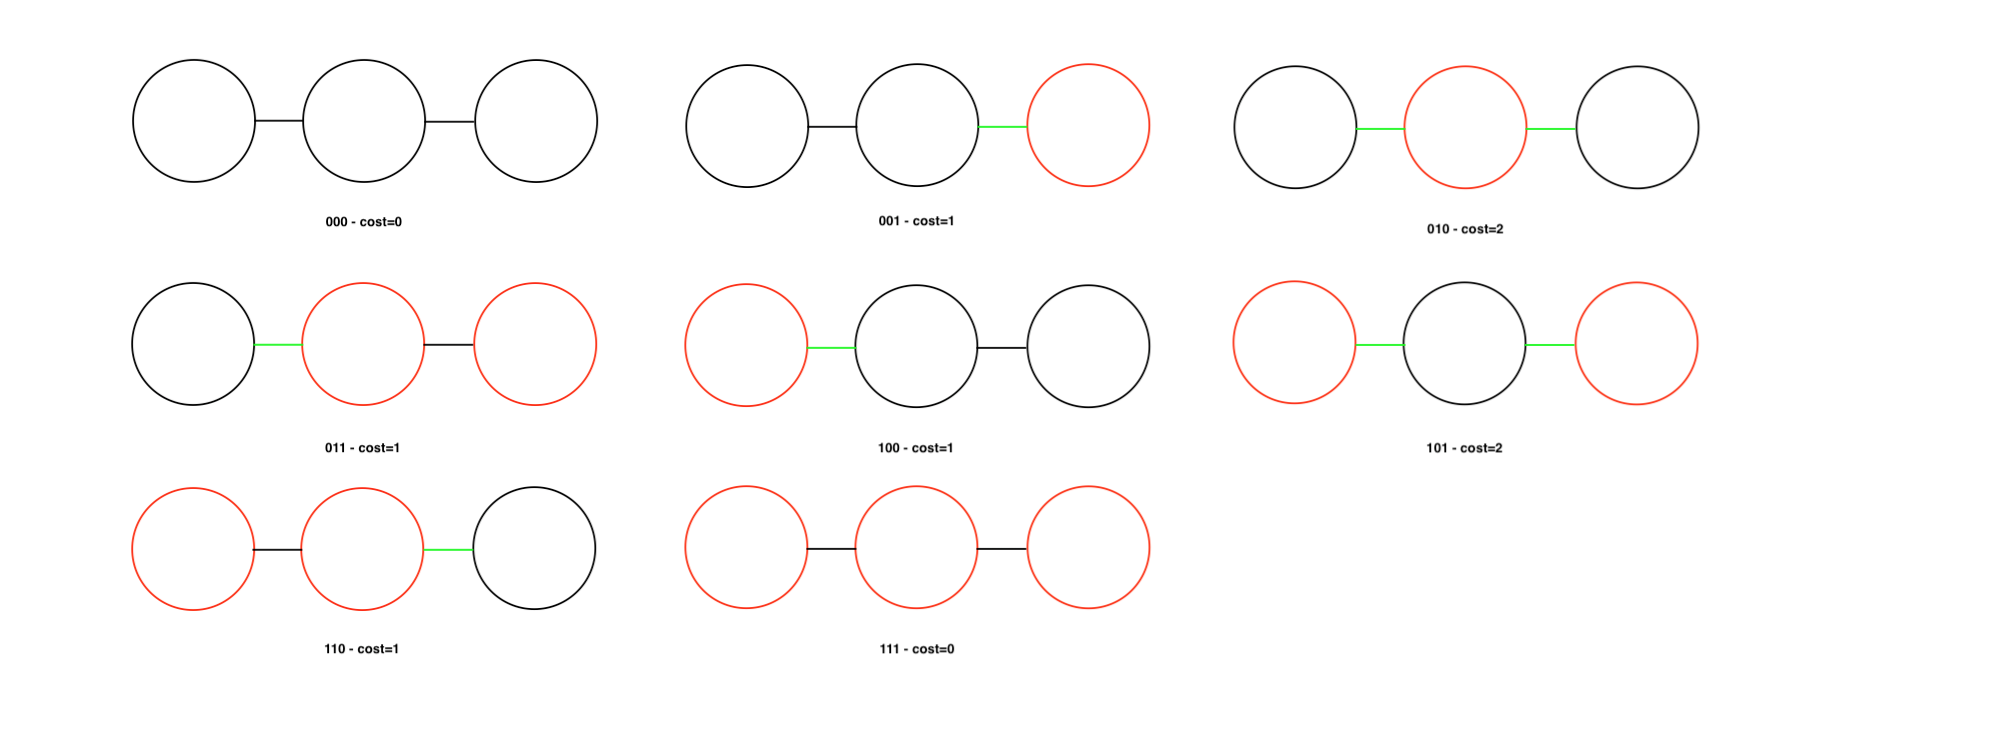
\includegraphics[width = \columnwidth]{fig/02_3_nodes_cuts.png}
    \caption{Max cut edge avec 3 noeuds}
    \label{fig:Max_cut_edge_3}
\end{figure}

On peut alors formuler le cout du problème comme suit:

\begin{equation}
    C_{total} = \sum C_{ij} = \sum \frac{1}{2} w_{ij} (1 - z_i z_j)
\end{equation}

avec $w_{ij} = 1$ si $i$ et $j$ sont reliés par une arête et $0$ sinon. $z_i$ et $z_j$ sont les variables binaires qui définissent si un noeud appartient à une coupe ou non.


\subsection{Encodage quantique du problème : Quel Hamiltonien ?}

Enfait, ce qui est agréable avec le Max Cut edge est que l'on peut facilement encoder le problème en un Hamiltonien d'Ising.
En effet, on peut associer un qubit à chaque noeud de notre graphe, et on peut associer un poids de couplage entre deux qubits si les deux noeuds sont reliés par une arête.

On peut alors définir l'Hamiltonien d'Ising comme suit :

\begin{equation}
    \hat{H} = -\sum_{i,j} J_{ij}\hat{\sigma}_i^z\hat{\sigma}_j^z - \sum_i h_i\hat{\sigma}_i^z
\end{equation}

Avec $\hat{\sigma}_i^z$ l'observable de Pauli, $J_{ij}$ les poids de couplage entre les spins et $h_i$ les champs magnétiques locaux.

On peut alors définir les poids de couplage comme suit :

\begin{equation}
    J_{ij} = \begin{cases} 1 & \text{si } i \text{ et } j \text{ sont reliés par une arête} \\ 0 & \text{sinon} \end{cases}
\end{equation}

Et les champs magnétiques locaux comme suit :

\begin{equation}
    h_i = 0
\end{equation}

En conclusion, le fait qu'un noeud appartient à une coupe ou non est donné par l'état de notre qubit est très pratique sinon on aurait du encoder cette information dans plusieurs qubits (analogie avec le bit classique).

\subsection{Implementation}


On va ainsi encoder notre problème en utilisant la librairie Leap et l'exécuter sur un ordinateur quantique D-Wave.

Pour être plus précis, D-Wave propose uniquement des annealers. Il n'y a donc pas de portes logiques et on peut seulement imposer la forme de l'hamiltonien auquel sont soumis nos qubits.
En fait, c'est uniquement ce dont nous avons besoin. Le code suivant repose sur des travaux antérieurs (\cite{jain_solving_2021}, \cite{stechly_mstechlyquantum_tsp_tutorials_2024}).

On formule d'abord notre problèmesous forme d'un graphe :

\begin{lstlisting}[language=Python]
    G = nx.Graph()
    G.add_edges_from([
        [0,3],[0,4],[1,3],[1,4],
        [2,3],[2,4],[3,5], [1,3],
        [6,7], [2,7], [5,7], [3,5]
        ])
    nx.draw(G, 
        pos=nx.bipartite_layout(
            G, [0,1,2]
            ))
\end{lstlisting}

On obtient la figure suivante :

\begin{figure}[H]
    \centering
    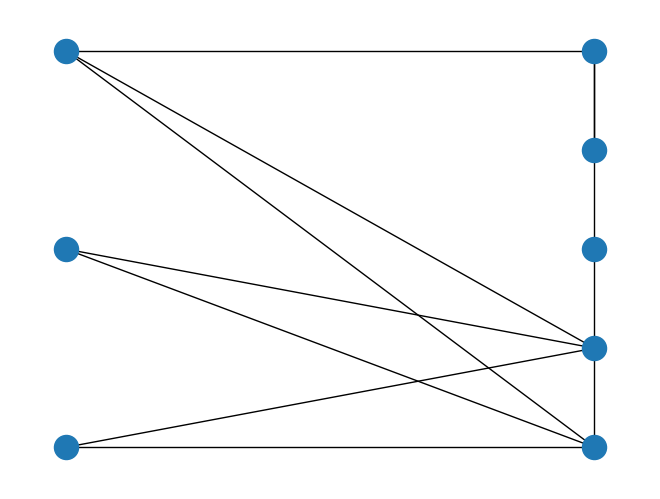
\includegraphics[width = \columnwidth]{fig/oriented_graph.png}
    \caption{Graphe du problème}
    \label{fig:Graph_problem}
\end{figure}

On transforme ensuite ce graphe en Mamiltonien d'Ising :

\begin{lstlisting}[language=Python]
    # Initialize our h vector, J matrix
    h = defaultdict(int)
    J = defaultdict(int)

    # Update J matrix 
    # for every edge in the graph
    for i, j in G.edges:
        J[(i,j)]+= 1
\end{lstlisting}

On crée ensuite une instance de sampler qui correspond à notre d'ordinateur quantique :

\begin{lstlisting}[language=Python]
    #  Run our QUBO on the QPU 
    client = Client.from_config(
        config_file="dwave.conf",
         profile="bqm")

    sampler = EmbeddingComposite(
        DWaveSampler()
        )
    
    # Set up QPU parameters
    chainstrength = 2
    numruns = 10
\end{lstlisting}

Finalement, on soumet l'hamiltonien à notre sampler, et il retourne la solution optimisé :

\begin{lstlisting}[language=Python]
    # Solve the problem
    response=sampler.sample_ising(h, J) 
\end{lstlisting}

On obtient alors la solution suivante :

\begin{table}[H]
    \centering
    \begin{tabular}{cccccccc}
        \hline
        0 & 1 & 2 & 3 & 4 & 5 & 6 & 7 \\
        \hline
        -1 & -1 & -1 & +1 & +1 & -1 & -1 & +1 \\
        +1 & +1 & +1 & -1 & -1 & +1 & +1 & -1 \\
        % \hline
        % \multicolumn{8}{c}{Energy: -10.0, Number of Occurrences: 10, Chain Strength: 0.0} \\
        % \hline
    \end{tabular}
    \caption{Coupe maximale du graphe}
    \label{tab:Solution}
\end{table}

On peut alors visualiser la solution :

\begin{figure}[H]
    \centering
    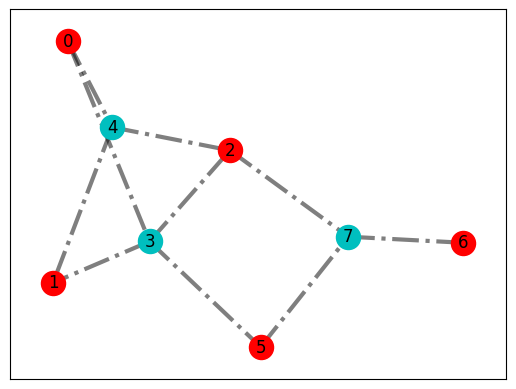
\includegraphics[width = \columnwidth]{fig/solution.png}
    \caption{Représentation de la coupe maximale du graphe}
    \label{fig:Graph_solution}
\end{figure}



\section{conclusion}

Ce projet bibliographique a permis de présenter les principes fondamentaux de l'informatique quantique, en particulier la notion de qubit, les différentes façons de les produire et les problèmes liés à leur utilisation. Le projet a également abordé la résolution d'un problème d'optimisation classique à l'aide d'un ordinateur quantique.

Les qubits, en tant qu'unités de base de l'information quantique, ont des propriétés uniques telles que la superposition et l'intrication, qui permettent d'effectuer des calculs de manière beaucoup plus efficace que les bits classiques. Cependant, la mesure d'un qubit est un processus irréversible qui détruit la superposition, ce qui rend la manipulation des qubits très délicate.

Pour produire des qubits, il existe plusieurs technologies prometteuses, notamment les qubits supraconducteurs, les qubits à ions piégés et les qubits à photons. Chacune de ces technologies a ses avantages et ses inconvénients en termes de stabilité, de scalabilité et de facilité de manipulation.

Le projet a également abordé la résolution d'un problème d'optimisation classique, le max cut edge, à l'aide d'un ordinateur quantique. Ce problème consiste à trouver la coupe d'un graphe qui maximise le nombre d'arêtes coupées. En utilisant un algorithme quantique, il est possible de trouver la solution optimale de manière beaucoup plus efficace que les algorithmes classiques.

En conclusion, l'informatique quantique est un domaine en pleine expansion qui offre des perspectives prometteuses pour la résolution de problèmes complexes. Cependant, la manipulation des qubits reste un défi majeur, et il est important de poursuivre les recherches pour améliorer la stabilité et la scalabilité des technologies de production de qubits. Le projet a permis de présenter les principes fondamentaux de l'informatique quantique et de montrer comment un ordinateur quantique peut être utilisé pour résoudre un problème d'optimisation.

\printbibliography

\end{multicols}



\end{document}